% ---------------------------------------------------
% ----- Main document of the template
% ----- for Bachelor-, Master thesis and class papers
% ---------------------------------------------------
%  Created by C. Müller-Birn on 2012-08-17, CC-BY-SA 3.0.
%  Last upadte: C. Müller-Birn 2015-11-27
%  Freie Universität Berlin, Institute of Computer Science, Human Centered Computing. 

\documentclass[pdftex,a4paper,12pt,DIV=calc,BCOR5mm,ngerman,twoside,smallheadings,titlepage]{scrbook}   
% ----- weitere Optionen 
%draft,			% Entwurfsmodus zum Anzeigen zu leerer/voller Boxen 
%DIV=calc
%DIV12,			% Seitengröße (siehe Koma Skript Dokumentation !) 
%BCOR5mm,		% Zusätzlicher Rand auf der Innenseite 
%twoside,		% Seitenränder werden an doppelseitig angepasst 
%fleqn,			% Formeln werden linksbündig (und nicht zentriert) angezeigt 
%titlepage,		% Titel wird in einer 'titlepage' Umgebung gesetzt 
%bigheadings,	% Große Überschriften (normal, small-headings) 
%halfparskip-	% Absatz wird nicht eingerückt, dafür aber um eine halbe Zeile nach unten gerückt
%
%---------------------------------------------------
%----- Packages
%---------------------------------------------------
%
\usepackage[T1]{fontenc} 
\usepackage[utf8]{inputenc}
\usepackage[ngerman]{babel} %\usepackage[english]{babel}  
\usepackage{ae} 
\usepackage{bibgerm}    

\usepackage{fancyhdr} % Define simple headings 
\usepackage{xcolor}
\usepackage{url}
\usepackage{listings}
%\usepackage{vmargin} % Adjust margins in a simple way
%
\usepackage{amsmath}
%
\usepackage[pdftex]{graphicx}  
\usepackage{hyperref} % turn all your internal references into hyperlinks
%\usepackage[pdfstartview=FitH,pdftitle={<<Titel der Arbeit>>}, pdfauthor={<<Autor>>}, pdfkeywords={<<Schlüsselwörter>>}, pdfsubject={<<Titel der Arbeit>>}, colorlinks=true, linkcolor=black, citecolor=black, urlcolor=black, hypertexnames=false, bookmarksnumbered=true, bookmarksopen=true, pdfborder = {0 0 0}]{hyperref}
%
% table settings 
\usepackage{booktabs}  
\usepackage{tabularx}  
\usepackage{rotating}
\usepackage{longtable}
\usepackage{pdflscape}
\usepackage{multirow} %multi row
\usepackage{rotating} %for rotating table
%
%---------------------------------------------------
%----- PDF and document setup
%---------------------------------------------------
%
\hypersetup{
	pdftitle={<My title>},  % please, add the title of your thesis
    pdfauthor={<Author>},   % please, add your name
    pdfsubject={<<Bachelor/Master thesis>, Institute of Computer Science, Freie Universität Berlin>}, % please, select the type of this document
    pdfstartview={FitH},    % fits the width of the page to the window
    pdfnewwindow=true, 		% links in new window
    colorlinks=false,  		% false: boxed links; true: colored links
    linkcolor=red,          % color of internal links
    citecolor=green,        % color of links to bibliography
    filecolor=magenta,      % color of file links
    urlcolor=cyan           % color of external links
}
% 
%---------------------------------------------------
%----- Customize page size
%---------------------------------------------------
\usepackage[top=3cm,right=3cm,bottom=4cm,left=4cm]{geometry}    
%
%---------------------------------------------------
%----- Customize header and footer\pagestyle{fancy} 
%---------------------------------------------------
\pagestyle{fancy}

\fancyhf{}  % delete all existing header formating

\fancyhead[LE]{\leftmark}  % represent the current chapter heading in uppercase
\renewcommand{\chaptermark}[1]{ % adapt the shown chapter name: show it in lower case and with chapter number 
\markboth{\thechapter.\ #1}{}}   

\fancyhead[RO]{\rightmark}   % % represent the current section heading in uppercase 
\renewcommand{\sectionmark}[1]{% adapt the shown section name: show it in lower case and with section number 
\markboth{\thesection.\ #1}{}}

\renewcommand{\headrulewidth}{0pt} % remove lines from header
\renewcommand{\footrulewidth}{0pt} % remove lines from header

\fancyfoot{} % delete all existing footer formating
\fancyfoot[LE,RO]{\thepage} % put page number on the left on even page and right on odd page
%
%---------------------------------------------------      
%----- Settings for word separation  
%---------------------------------------------------      
% Help for separation (from package babel, section 22)):
% In german package the following hints are additionally available:
% "- = an explicit hyphen sign, allowing hyphenation in the rest of the word
% "| = disable ligature at this position. (e.g., Schaf"|fell)
% "~ = for a compound word mark without a breakpoint (e.g., bergauf und "~ab)
% "= = for a compound word mark with a breakpoint, allowing hyphenation in the composing words
% "" = like "-, but producing no hyphen sign (e.g., und/""oder)
%
% Describe separation hints here:
\hyphenation{
% Pro-to-koll-in-stan-zen
% Ma-na-ge-ment  Netz-werk-ele-men-ten
% Netz-werk Netz-werk-re-ser-vie-rung
% Netz-werk-adap-ter Fein-ju-stier-ung
% Da-ten-strom-spe-zi-fi-ka-tion Pa-ket-rumpf
% Kon-troll-in-stanz
}
%
%---------------------------------------------------
%----- Restricting including files   
%---------------------------------------------------
% Only files listed here will be included in the PDF document!
% In order to only partially translate the document, for example for bug-fixing, 
% it might be useful to comment out some of the documents.
\includeonly{
title,
declaration,
abstract_en,
abstract_de,
preface,
introduction,
chapters,
conclusion,
appendix
}

%%%%%%%%%%%%%%%%%%%%%%%%%%%%%%%%%%%%%%%%%%%%%%%%%%%%%%
% The content part of the documentent starts here! %%
%%%%%%%%%%%%%%%%%%%%%%%%%%%%%%%%%%%%%%%%%%%%%%%%%%%%%%

\begin{document}
%---------------------------------------------------
%----- Listing and color definition   
%---------------------------------------------------
\definecolor{red}{rgb}{.8,.1,.2}
\definecolor{blue}{rgb}{.2,.3,.7}
\definecolor{lightyellow}{rgb}{1.,1.,.97}
\definecolor{gray}{rgb}{.7,.7,.7}
\definecolor{darkgreen}{rgb}{0,.5,.1}
\definecolor{darkyellow}{rgb}{1.,.7,.3}
\lstloadlanguages{C++,[Objective]C}
\lstset{
		escapeinside={§§}{§§},
        basicstyle=\ttfamily\footnotesize\mdseries,
        columns=fullflexible,% typewriter font look better with fullflex
        keywordstyle=\bfseries\color{blue},
%		identifierstyle=\bfseries,
        commentstyle=\color{darkgreen},      
        stringstyle=\color{red},
        numbers=left,
        numberstyle=\ttfamily\scriptsize\color{gray},
%       stepnumber=5,
%       numberfirstline=true,
        breaklines=true,
%		prebreak=\\,
        showstringspaces=true,
        tabsize=4,
        captionpos=b,
%		framexrightmargin=-.2\textwidth,
        float=htb,
		frame=tb,
		frameshape={RYR}{n}{n}{RYR},
		rulecolor=\color{darkyellow},
        xleftmargin=15pt,
        xrightmargin=4pt,
        aboveskip=\bigskipamount,
        belowskip=\bigskipamount,
		backgroundcolor=\color{lightyellow},
		extendedchars=true,
       	belowcaptionskip=15pt
}

%---------------------------------------------------
%----- Title and declaration   
%---------------------------------------------------
\pagenumbering{alph} % even though, these page numbers are not visible there are necessary to have unique page numbers 
% ---------------------------------------------------
% ----- Title page of the template
% ----- for Bachelor-, Master thesis and class papers
% ---------------------------------------------------
%  Created by C. Müller-Birn on 2012-08-17, CC-BY-SA 3.0.
%  Freie Universität Berlin, Institute of Computer Science, Human Centered Computing. 
%
\begin{titlepage}

\title{
\includegraphics[width=0.6\textwidth]{pics/FU_logo.pdf}\\
{\small Bachelorarbeit am Institut für Informatik der Freien Universität Berlin}\\
{\small Human-Centered Computing (HCC)}\\
[6ex]
{\LARGE Comparing interpretability techniques for unsupervised topic modeling}}

\author{
{\emph{\normalsize Tim Korjakow}}\\
{\normalsize Matrikelnummer: 372862}\\
{\normalsize Email: tim.korjakow@campus.tu-berlin.de}\\ 
[18ex]   
{\normalsize Betreuer: Jesse Jonas Benjamin} \\
{\normalsize Betreuerin und Erstgutachterin: Prof. Dr. C. Müller-Birn} \\
{\normalsize Zweitgutachter: Prof. Dr. K. Müller}}
\vspace{6ex}
\date{\normalsize Berlin, 08.08.2019}
 
\maketitle  

\end{titlepage}
% ---------------------------------------------------
% ----- Declaration of the template
% ----- for Bachelor-, Master thesis and class papers
% ---------------------------------------------------
%  Created by C. Müller-Birn on 2012-08-17, CC-BY-SA 3.0.
%  Freie Universität Berlin, Institute of Computer Science, Human Centered Computing. 
%
\pagestyle{empty}

\subsection*{Eidesstattliche Erklärung}

Ich versichere hiermit an Eides Statt, dass diese Arbeit von niemand anderem als meiner Person verfasst worden ist. Alle verwendeten Hilfsmittel wie Berichte, Bücher, Internetseiten oder ähnliches sind im Literaturverzeichnis angegeben, Zitate aus fremden Arbeiten sind als solche kenntlich gemacht. Die Arbeit wurde bisher in gleicher oder ähnlicher Form keiner anderen Prüfungskommission vorgelegt und auch nicht veröffentlicht.
\par\bigskip  
\noindent Berlin, den \today

\vspace{1.2cm}

\noindent <Name>  

\cleardoublepage

%---------------------------------------------------
%----- Abstracts in English and German   
%---------------------------------------------------

% ---------------------------------------------------
% ----- Abstract (English) of the template
% ----- for Bachelor-, Master thesis and class papers
% ---------------------------------------------------
%  Created by C. Müller-Birn on 2012-08-17, CC-BY-SA 3.0.
%  Freie Universität Berlin, Institute of Computer Science, Human Centered Computing. 
%
\pagestyle{empty}

\subsection*{Abstract}

<Please summarize your thesis in a brief but meaningful way (about one page). Include in your abstract the topic of this thesis, important contents, results of your research and an evaluation of your results.>

\cleardoublepage

% ---------------------------------------------------
% ----- Abstract (German) of the template
% ----- for Bachelor-, Master thesis and class papers
% ---------------------------------------------------
%  Created by C. Müller-Birn on 2012-08-17, CC-BY-SA 3.0.
%  Freie Universität Berlin, Institute of Computer Science, Human Centered Computing. 
%
\pagestyle{empty}

\subsection*{Zusammenfassung}

<Hier sollten Sie eine kurze, aussagekräftige Zusammenfassung (ca. eine Seite) Ihrer Arbeit geben, welche das Thema der Arbeit, die wichtigsten Inhalte, die Arbeitsergebnisse und die Bewertung der Ergebnisse umfasst.> 

\cleardoublepage  
                                          
%---------------------------------------------------
%----- Directories   
%---------------------------------------------------

\frontmatter 
\pagenumbering{roman}

\tableofcontents
\setcounter{tocdepth}{3}   % reduce the included sections in the table of content

\listoffigures
\listoftables

%---------------------------------------------------
%----- Main part
%---------------------------------------------------
\mainmatter
\pagenumbering{arabic} 
\pagestyle{fancy} 

% ---------------------------------------------------
% ----- Preface of the template
% ----- for Bachelor-, Master thesis and class papers
% ---------------------------------------------------
%  Created by C. Müller-Birn on 2012-08-17, CC-BY-SA 3.0.
%  Freie Universität Berlin, Institute of Computer Science, Human Centered Computing. 
%
\chapter*{Vorwort}
\label{chap:preface}

\section*{Allgemeine Hinweise zur Erstellung einer Abschlussarbeit}

\begin{itemize}
	\item Beachten Sie, dass diese Vorlage für einen zweiseitigen Ausdruck angelegt wurde.  
	\item Über die Papierqualität können Sie entscheiden, aber wir empfehlen aber Seiten mit wichtigen, farbigen Grafiken auch in Farbe auszudrucken und dabei ein höherwertiges Papier zu verwenden. 
	\item Bitte stimmen Sie mit dem Betreuer Ihrer Arbeit auch den Zweitgutachter ab. Die Anfrage des Zweitgutachters erfolgt von Ihnen. Es ist an dieser Stelle sinnvoll, die Anfrage mit einer kurzen Zusammenfassung der Arbeit zu stellen.  
	\item Bitte beachten Sie, dass Sie Ihre Abschlussarbeit mit einer Klebebindung versehen, eine Ringbindung ist nicht erwünscht. 
\end{itemize} 

% ---------------------------------------------------
% ----- Introduction of the template
% ----- for Bachelor-, Master thesis and class papers
% ---------------------------------------------------
%  Created by C. Müller-Birn on 2012-08-17, CC-BY-SA 3.0.
%  Last upadte: C. Müller-Birn 2015-11-27 
%  Freie Universität Berlin, Institute of Computer Science, Human Centered Computing. 
%
\chapter{Thematic Introduction and Motivation}
\label{chap:introduction}

\section{Project IKON}

This thesis has a direct application in a project which tries to explore potentials for knowledge transfer activities at a research museum. Project \textit{IKON} was started in cooperation with the German Natural History Museum in Berlin which houses more than 300 scientists, PhD students and other staff \cite{Team2018}. With that size of scientific staff the institution is a global player in research on evolution and biodiversity \cite{IntroducingMuseumFur}. Despite its importance in the research landscape, the museum is challenged with a lack of shared knowledge across working groups and organizational structures such as departments. In interviews researchers from the project were able to trace these problems back to the very intricate and complex layout of rooms and halls in the building which was originally constructed in 1810 \cite{140JahreAltes2018}. In order to mitigate this problem \autoref{pic:IKON-clusterview} shows one of the main deliverables of \textit{IKON} - a ML-driven data visualization which follows the path of knowledge at this research museum from its creation in projects over knowledge transfer activities, where multiple projects exchange their findings, to the final target group. Potentials for knowledge exchange are made explicit by visualizing projects not in the predefined taxonomy of the museum, but instead in semantic relation to each other. This is accomplished by running all project abstracts through a topic modeling process consisting of four major components, as seen in \autoref{pic:general_topic_extraction_pipeline}. 

\section{Topic modeling}

A generic topic modeling pipeline consists of four steps: 
\begin{enumerate}
	\item Document embedding
	\item Topic extraction
	\item Classification of documents
	\item Reduction into 2D
\end{enumerate}

Given an unlabeled corpus $C = \{D_1, ..., D_n\}$ consisting of $n$ documents $D_i = (t_1, ..., t_m)$, which in turn consists of a sequence of $m$ strings, also called tokens or words, the document embedding step assigns to each document a vector $v_D \in \mathbb{R}^e, e \in \mathbb{N}^+$. Semantically similar documents should also be closer in the embedded vector space with respect to a given distance measure than documents which are semantically not related. Therefore this step transforms a corpus into a matrix $(v_1, ..., v_n) \in \mathbb{R}^{e \times n}$.

Consuming the output from the previous step the topic extraction tries to uncover $k$ latent structures. We call these structures \textit{topics}. Mathematically speaking a topic is a probability distribution over a fixed set of input features. \cite{liuOverviewTopicModeling2016} These features can correspond to tokens, as it is the case in the later discussed Tfidf-BOW embedding, but this does not have to be the case. Therefore this step transforms the corpus from the embedding space of dimensionality $e \times n$, where each document is described as linear combination of features, to the latent space of dimensionality $k \times n$, where each document is described as a linear combination of latent topics. Since most often $k < e$ holds true, this can also be seen as a form of dimensionality reduction, which is again a form of feature extraction.

Using the document vectors in the latent space each document is assigned a label. This may happen in a supervised way if there are labels available for training purposes, but in most cases an unsupervised classification, also known as clustering, is used to group the documents.

Finally in order to visualize the high dimensional distribution of documents in the latent space another dimensionality reduction is used to project the documents to 2D.

\begin{figure}[t]
	\centering
	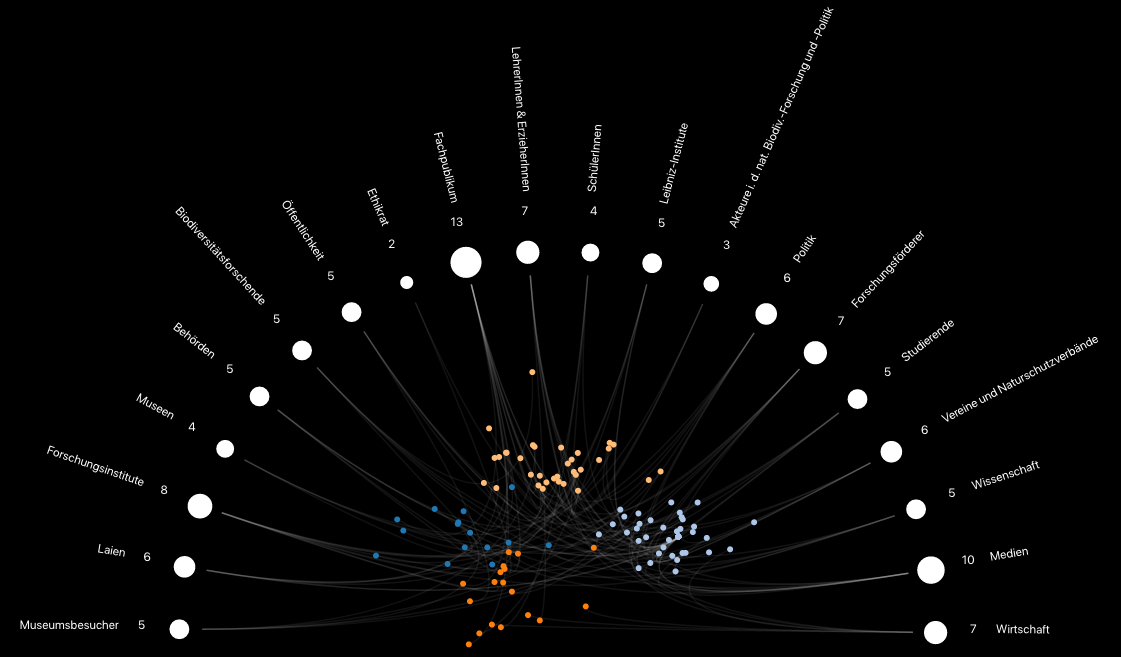
\includegraphics[width=400px]{../chapters/introduction/graphics/ikon-clusterview}
	\caption{\label{pic:IKON-clusterview} Screenshot of the cluster view of the IKON visualization}
\end{figure}

% Define block styles
\tikzstyle{decision} = [diamond, draw, fill=blue!20, 
text width=4.5em, text badly centered, node distance=3cm, inner sep=0pt]
\tikzstyle{block} = [rectangle, draw, fill=blue!20, 
text width=6.5em, text centered, rounded corners, minimum height=4em]
\tikzstyle{line} = [draw, -latex']
\tikzstyle{cloud} = [draw, ellipse,fill=red!20, node distance=3cm,
minimum height=2em]
\usetikzlibrary{decorations.text}

\begin{figure}[t]
	\centering
	\begin{tikzpicture}[node distance = 4cm, auto]
	% Place nodes
	\node [block] (emb) {Document embedding};
	%\node [cloud, left of=emb] (expert) {expert};
	%\node [cloud, right of=emb] (system) {system};
	\node [block, right of=emb] (topic) {Topic extraction};
	\node [block, right of=topic, above of=topic] (cluster) {Classification of documents};
	\node [block, right of=topic, below of=topic] (2D) {Reduction into 2D};
	% Draw edges
	\path [line] (emb) -- (topic);
	\path [line] (topic) -- (cluster);
	\path [line] (topic) -- (2D);
	%\path [line] (identify) -- (evaluate);
	%\path [line] (update) |- (identify);
	%\path [line,dashed] (system) |- (evaluate);
	\end{tikzpicture}
	\caption{\label{pic:general_topic_extraction_pipeline} Components of a general topic extraction pipeline}
\end{figure}

Each component in \autoref{pic:general_topic_extraction_pipeline} comes with its own set of parameters which influence the results generated by the pipeline. Therefore the researchers from project IKON hypothesize, based in first interviews and conceptual work, that the museum's staff, as non-technical experts without knowledge of the capabilities and shortcomings of the models used in topic modeling, will have a hard time interpreting and understanding the output generated by the pipeline. 

In order to lay the groundwork for this thesis and understand the challenges which scientists face while interacting with the visualization I carried out an exploratory workshop with the researchers from project \textit{IKON}. In the beginning I asked them which kind of hardships they, based on their past experiences and interviews, hypothesize during the interaction between user and visualization. Followed by an explanation of \autoref{pic:general_topic_extraction_pipeline} we discussed how these challenges may correlate with goals and questions. Following a description of the key questions each question was categorized according to the pipeline step, as seen in \autoref{tab:overview_viz_questions}, which may contribute information in order to support the user in answering his question.

\begin{table}
	\centering
	\begin{tabular}{ c | c }
		\hline 
		Question & Applicable pipeline component \\ \hline
		How does the research landscape look like \\ and on what kind of topics are prominent? & Topic Extraction \\ \hline
		What does a cluster mean? & Classification \\ \hline
		What does the distance between \\ clusters/projects mean? & Topic Extraction / Reduction into 2D \\ \hline
		How similar are two projects/clusters? & Topic Extraction \\
		\hline
	\end{tabular}
	\caption{\label{tab:overview_viz_questions} Table showing the sourced questions and the pipeline step which could provide an answer}
\end{table} 

\section{Interpretability}

In the same workshop we also developed a way of structuring commonly used terminology in the field of explainability/interpretability research, where terms explainability and interpretability are commonly used as synonyms. Our notion builds upon the findings of Miller and Lipton, which concluded that, interpretability as term has become an ill-defined objective \cite{liptonMythosModelInterpretability2016a} for research and development in ML algorithms since there is no widely agreed upon definition of it. This leads to a very fragmented nature of the field. Furthermore Miller et al. \cite{millerExplainableAIBeware2017} support this point by conducting a literature study and uncovering that interpretability research is rarely influenced by insights from the humanities, especially connected fields as explainability or causality research.

Therefore the researchers from project IKON propose that the context in which interpretation is performed is essential to the outcome of the interpretative process. In this discussion the term 'context' considers the situational context of the interaction between user and system as well as the historical experiences of the user. They introduce a relational model in which users posses a set of \textit{a priori} preferred explanation strategies (e.g. comparing two entities) given the context of the interaction and their previous experiences. As a consequence of having this preferred set, they only consider a specific subset of all possible types of explanations as valid. Interpretability techniques on the other hand are conditioned in regard to an algorithmic system, e.g. a specific model or class of models. These techniques can be described by algorithms and deliver concrete explanations given a model and a model output. Therefore a interpretability technique serves as the missing link between high-level explanation strategies, an algorithmic system and explanations.
 

\begin{figure}[t]
	\centering
	\begin{tikzpicture}[node distance = 6cm, auto]
	% Place nodes
	\node [block] (strat) {Explanation strategy};
	\node [block, right of=strat] (expl) {Explanation};
	\node [block, below of=strat] (alg) {Algorithmic system};
	\node [block, below of=expl] (int) {Interpretability technique};
	% Draw edges
	\path [line,dashed,
	postaction={decorate},
	decoration={text along path,
		text=requires,
		text align={left indent={0.2\dimexpr\pgfdecoratedpathlength\relax}}
	}] 
	(strat) -- (expl);
	
	\path [line,
	postaction={decorate},
	decoration={text along path,
		text=instantiates,
		text align={left indent={0.2\dimexpr\pgfdecoratedpathlength\relax}}
	}] 
	(int) -- (strat);
	
	\path [line,
	postaction={decorate},
	decoration={text along path,
		text=produces,
		text align={left indent={0.2\dimexpr\pgfdecoratedpathlength\relax}}
	}]
	(int) -- (expl);
	
	\path [line,
	postaction={decorate},
	decoration={text along path,
		text=conditions,
		text align={left indent={0.2\dimexpr\pgfdecoratedpathlength\relax}}
	}] 
	(alg) -- (int);
	\end{tikzpicture}
	\caption{\label{pic:interpretability_relational} Relational model showing the interplay of explanation strategies, interpretability techniques and explanations}
\end{figure}

\section{Working plan}
In order to research how these interpretability techniques could be applied in project IKON, I will conduct the following three steps:

\begin{enumerate}
	\item Since I as a developer did not possess an exhaustive list of techniques to enhance explainability for unsupervised NLP models exist, a thorough and reproducible literature analysis on the status of XAI research in the field of NLP according to Petersen et al. \cite{petersenSystematicMappingStudies2008a} is going to be conducted. This should result in a number of papers which are, according to the process, good representatives of the literature base and therefore also of current research efforts. A quantitative analysis of these papers should summarize occurring XAI methods and categorize them according to an applicable categorization. 
	
	\item The currently existing topic extraction pipeline can be generalized into the following four components: document embedding, dimensionality reduction into a topic space, clustering and another dimensionality reduction into 2D. Based on the results of the previous step for each component either a directly applicable method (e.g. a clustering algorithm) from a paper or a model which supports most collected methods (e.g. a neural network for document embedding) is chosen and implemented. Since the new pipeline should capture at least as much information as the old one, each component will be quantitatively accessed according to applicable measures e.g. (\cite{roderExploringSpaceTopic2015a}). This is necessary to ensure that one is actually interpreting existing and captured semantic relations and not random artifacts generated by the various methods.
	
	\item A full user study would normally be necessary to assess how the implemented methods may support a non-technical expert in interpreting the results of the pipeline, but in order to keep the volume of this thesis in a feasible frame I will resort to a cognitive walkthrough from the point of view of a researcher from the national natural history museum.
	Since ensuring robustness in such qualitative tests is always a concern, information from previous interviews with domain experts from the museum will be used to derive meaningful tasks. The walkthrough should show how the implemented techniques may help with answering the initially sourced questions from step 1.
\end{enumerate}


% ---------------------------------------------------
% ----- Chapters of the template
% ----- for Bachelor-, Master thesis and class papers
% ---------------------------------------------------
%  Created by C. Müller-Birn on 2012-08-17, CC-BY-SA 3.0.
%  Freie Universität Berlin, Institute of Computer Science, Human Centered Computing. 
%
\chapter{Kapitel}
\label{chap:chapters} 

\begin{itemize}
	\item Abhängig vom Ziel der Arbeit und dem verwendeten Forschungsdesign unterscheidet sich dieser Hauptteil der Arbeit erheblich. 
	\item Eine sehr allgemeine Struktur ist die folgende:
	\begin{itemize}
		\item Hintergrund der Arbeit (Theoretische Einordnung der Arbeit) 
		 	\begin{itemize}
		 		\item Hier sollte enthalten sein, welche Anwendungen in diesem Bereich bereits existieren und warum bei diesen ein Defizit besteht. 
				\item Falls genutzt, sollten hier die entsprechenden Algorithmen erläutert werden.
				\item Es sollten die Ziele der Anwendungsentwicklung, d.h. die Anforderungen herausgearbeitet werden. Dabei sollte die bestehende Literatur geeignet integriert werden.
		 	\end{itemize}
		\item Umsetzung (Praktischer Anteil der Arbeit)
			\begin{itemize}
				\item Zunächst sollte die Softwarearchitektur und die genutzten Anwendungen, APIs etc. erläutert werden. Ebenfalls gehört dazu das Datenbankschema.
				\item Es sollten die zentralen Elemente der Software (abhängig von der Aufgabenstellung) beschrieben werden, wie implementierte Algorithmen oder das Oberflächendesign.
				\item Zentraler Quellcode sollte entsprechend aufgelistet werden:
				\lstset{language=Java,basicstyle=\footnotesize,numbers=left,showstringspaces=false,frame=single}
				\begin{lstlisting}
				public class Main {
					public static void main(String[] args) {
						System.out.println("Hello World!");
					}
				}
				\end{lstlisting} 
				%\item Klassendiagramm für Backend
				%\item Dr Quellcode zentraler Implementierungen  können als Auszug in den Anhang. Im Text kann dann darauf verwiesen werden.
			\end{itemize}
		\item Evaluation (zumeist nur für Masterarbeiten relevant)
		\begin{itemize}
			\item Jede Software muss auch getestet werden. Dieses Tests werden entweder mit einem vorgegebenen Datensatz erfolgen oder aber die Evaluation erfolgt auf Basis von Experimenten. In diesem Kapitel sollte daher entweder der genutzte Datensatz oder der experimentelle Aufbau beschrieben werden. 
		\end{itemize}
		\item Ergebnis und Diskussion
		\begin{itemize}
			\item Die Ergebnisse der Anwendung werden in diesem Kapitel vorgestellt und anschließend diskutiert. Wenn möglich sollte die Ergebnisse in Relation zu bestehenden Arbeiten in dem Bereich erörtert werden.
		\end{itemize}
	\end{itemize}  
\end{itemize}

\chapter{Literature mapping study}

\section{Motivation}

\section{Methodology}
In order to generate a reproducible and current overview over the fast-moving field of interpretability research in machine learning a rigorous methodology by Peterson et al. \cite{petersenSystematicMappingStudies} is used. 

The recommended process is augmented by further steps in order to tailor it to the existing use case and consists of the following seven procedures:
\begin{enumerate}
	
	\item Definition of research questions:
	
	The first step is the most crucial one as the questions defined here guide the development of the whole literature study and subsequently the result as well. The questions should 
	
	\item Construction of a search string
	
	Based on the questions one is able to gather a set of key words which are most relevant to the field which is analyzed. Each word is augmented by synonyms which are most often used
	\item Analysis of the main publishers using a meta search using the search string
	\item Sourcing of publications in scientific databases
	\item Filtering of these publications by keywording their abstracts
	\item Definition of inclusion and exclusion criteria to narrow down the pool of publications further
	\item Quantitative and qualitative assessment of the resulting corpus
\end{enumerate}

The overall process starts by defining clear questions which should guide 
% ---------------------------------------------------
% ----- Conclusion of the template
% ----- for Bachelor-, Master thesis and class papers
% ---------------------------------------------------
%  Created by C. Müller-Birn on 2012-08-17, CC-BY-SA 3.0.
%  Freie Universität Berlin, Institute of Computer Science, Human Centered Computing. 
%
\chapter{Conclusion}
\label{chap:conclusion}

As stated in the Introduction, this thesis was conducted in order to study what kind of explainability techniques for NLP exist and how they could support a non-technical expert in understanding the output from the system.

The first step was a systematic literature mapping study according to Petersen et al. \cite{petersenSystematicMappingStudies} which unveiled that I was able to confirm the findings of Lipton \cite{liptonMythosModelInterpretability2016a} and Miller \cite{millerExplanationArtificialIntelligence2017} in the domain of NLP.
Furthermore the results from the literature mapping study suggest that most of the current research focuses on supervised methods, such as neural networks, and these models are mainly made interpretable through local instance explanations. A proper definition of interpretability or an analysis of how a method influences interpretability lacks in a majority of publications on the other hand.

Based on these findings I was now able to take each component of the general topic extraction pipeline in \autoref{pic:general_topic_extraction_pipeline} and propose and implement a contending method. Each method was evaluated according to standard measures in order to ensure proper performance. Three out of four components where also augmented by explainability methods, while none of these techniques was implemented directly from one of the sourced papers, because none was able to answer the questions I formulated in the beginning and also .
Following an analysis investigating the interplay between all implemented methods, the decision was made to remain with the existing pipeline, but augment it by the proposed explainability techniques.

A cognitive walkthrough simulating a researcher doing an exploratory interaction unveiled a number of usability issues, but also showed how the implemented techniques support the user in making inferences about the output of the topic modeling pipeline.  

\section{Outlook}   
As discussed in \autoref{chap:literature_analysis} and visible in the results of the literature mapping study, there are a number of additional explanation strategies which could be applied to the augmented topic modeling pipeline.

Although the performance of Agglomerative Clustering didn't seem to satisfy the needs of the application, the idea of explaining a model by an induced taxonomy is still very interesting \cite{Liu:2018:INE:3219819.3220001}. Factoring in that the majority of the staff at the museum are trained biologists and taxonomies are widely used in this scientific discipline, these structures may be a very useful metaphor to present information to these non-technical experts.

Furthermore during the work on this thesis another potential question, additional to the ones defined in \autoref{tab:overview_viz_questions}, arose:
\begin{center}
	What kind of potential projects exist in the space between projects?
\end{center}
One of the already used techniques could be used to deliver potential answers . If the current LDA reduction gets replaced by a special kind of autoencoding, called variational autoencoding (VAE), it should be possible to generate meaningful vectors in the latent topic space and via the previously discussed methods also top words for these potential projects. 

Asides from additional explainability strategies and further model tuning, the whole system needs to be subjected to complete and rigorous user test with non-technical experts from the museum. The cognitive walkthrough included in this thesis does deliver a few insights into the usability of the application and the interaction with the topic modeling pipeline, but only a test in the situational context of the environment of the museum can convey reliable information concerning the interpretability of the used algorithms and the inferences the users are able to make using the system.



%---------------------------------------------------
%----- Bibliography
%---------------------------------------------------
\phantomsection
\addcontentsline{toc}{chapter}{Literatur}
\bibliographystyle{alpha}
\bibliography{references.bib,../../references/thesis/main.bib}

%---------------------------------------------------
%----- Appendix   
%---------------------------------------------------
\backmatter
% ---------------------------------------------------
% ----- Appendix of the template
% ----- for Bachelor-, Master thesis and class papers
% ---------------------------------------------------
%  Created by C. Müller-Birn on 2012-08-17, CC-BY-SA 3.0.
%  Freie Universität Berlin, Institute of Computer Science, Human Centered Computing. 
%

\chapter{Appendix}
\label{ch:Appendix}

\begin{figure}[t]
	\centering
	\includegraphics[angle=90,origin=c,width=330px]{/home/tim/HCC/IKON-backend/src/topicextraction/nlp/nlpflowchart_old}
	\caption{\label{pic:IKON_pipeline} BPMN process diagram of the existing topic modeling pipeline}
\end{figure}

\begin{figure}[t]
	\centering
	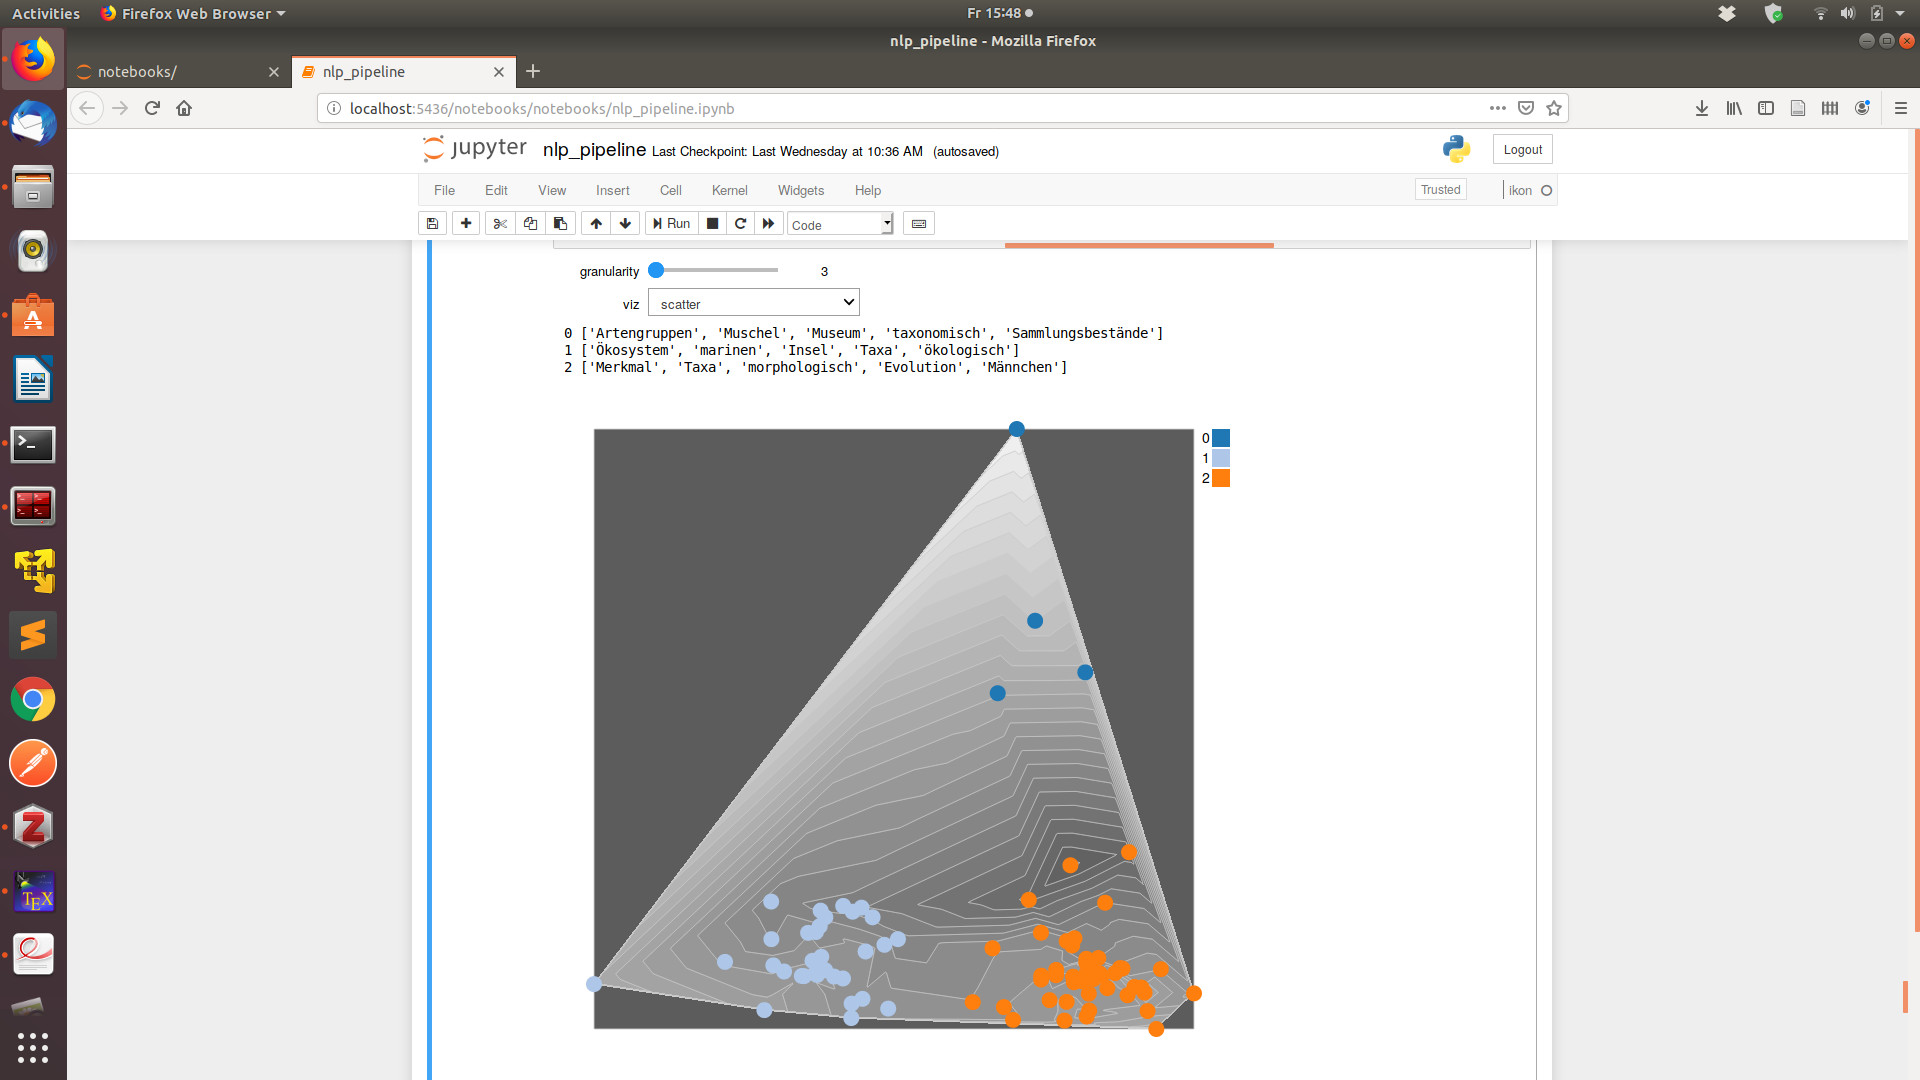
\includegraphics[width=400px]{../chapters/validation/pics/1}
	\caption{\label{pic:step1} Cognitive Walkthrough step 1}
\end{figure}

\begin{figure}[t]
	\centering
	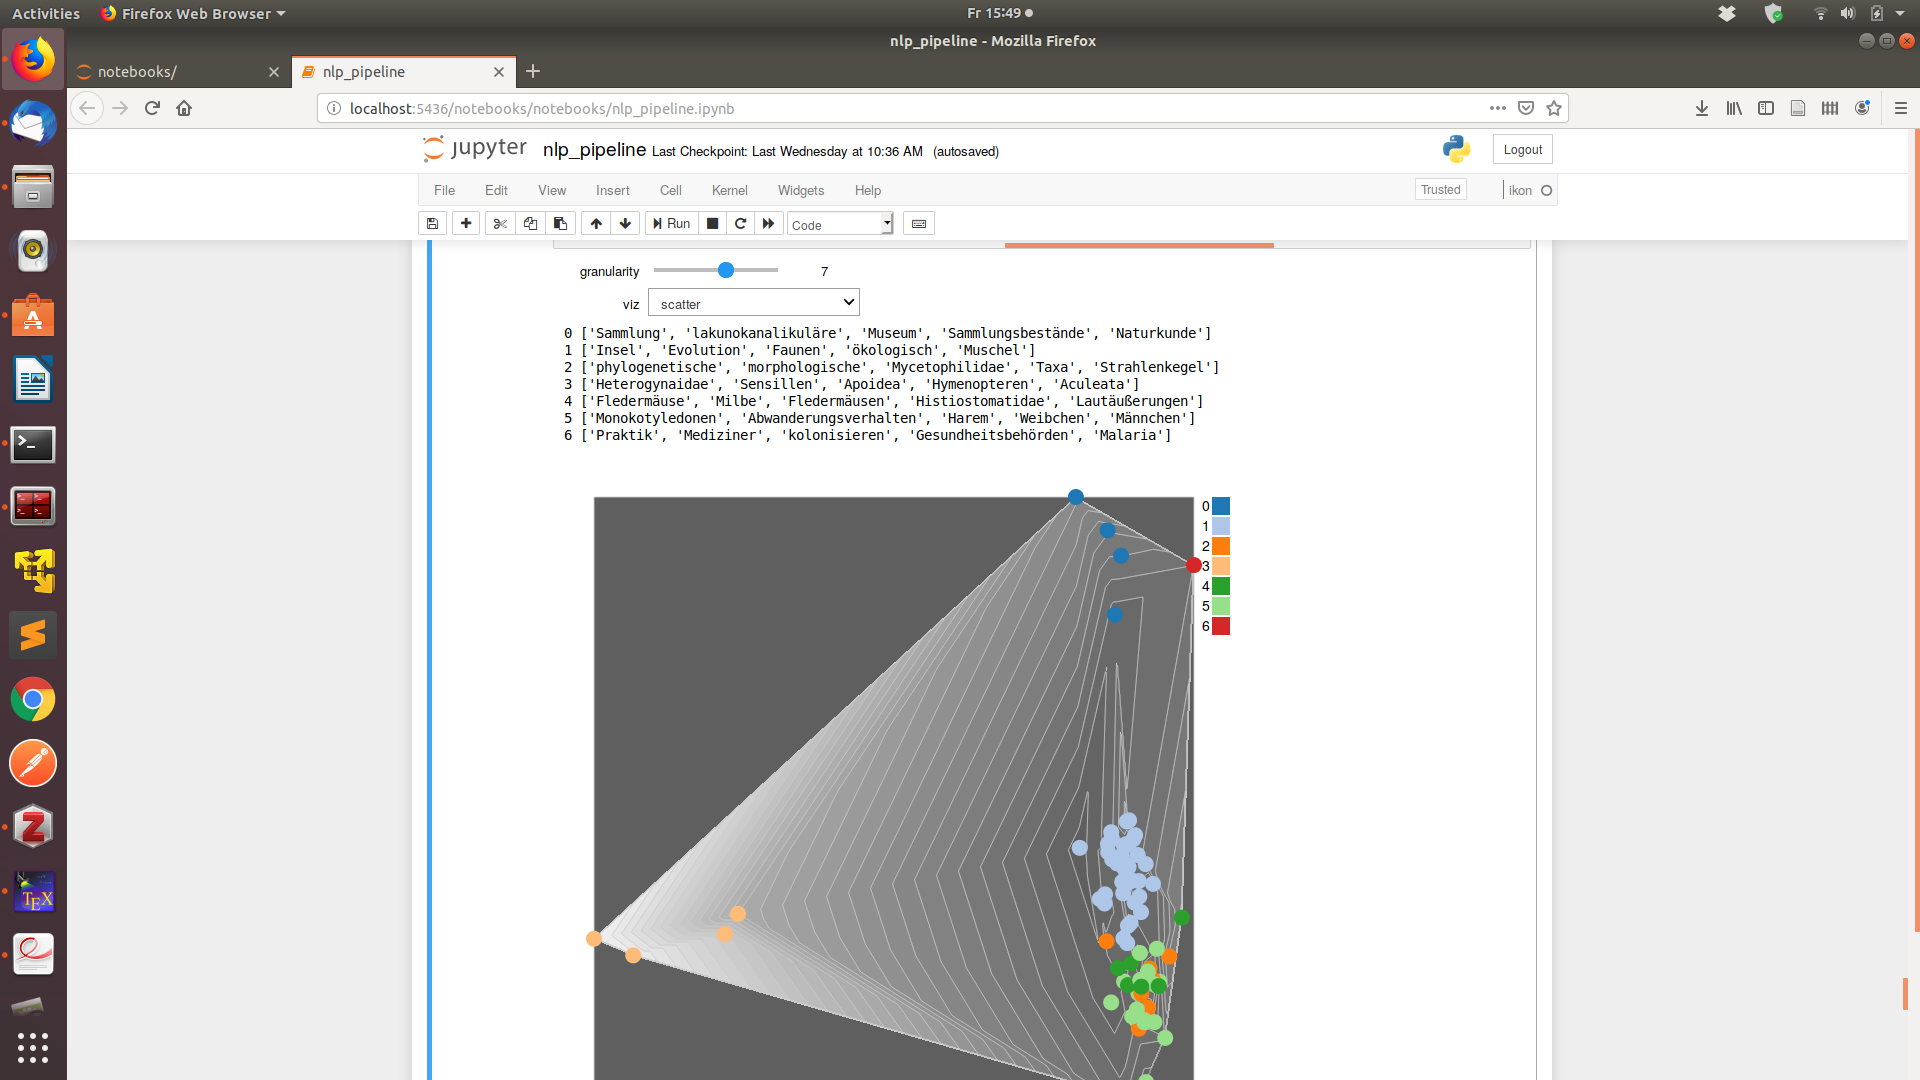
\includegraphics[width=400px]{../chapters/validation/pics/2}
	\caption{\label{pic:step2} Cognitive Walkthrough step 2}
\end{figure}

\begin{figure}[t]
	\centering
	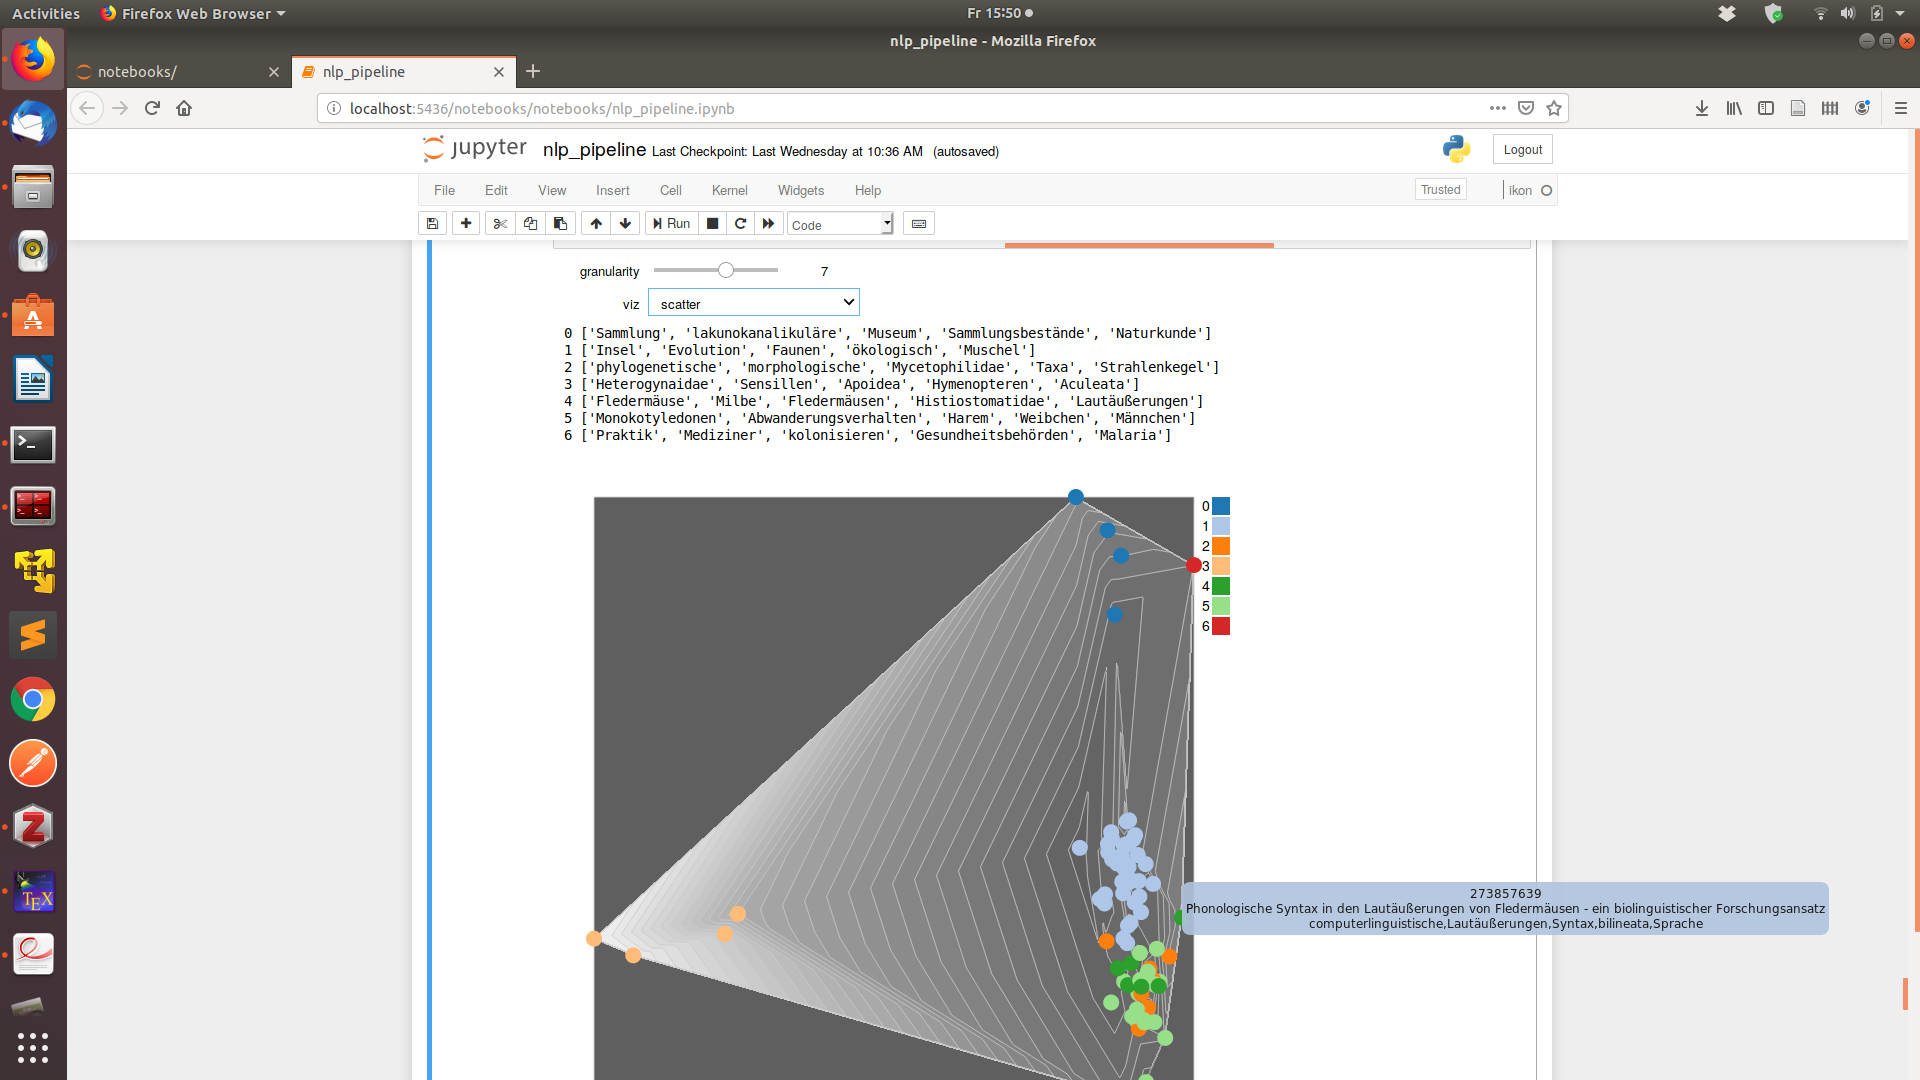
\includegraphics[width=400px]{../chapters/validation/pics/3}
	\caption{\label{pic:step3} Cognitive Walkthrough step 3}
\end{figure}

\begin{figure}[t]
	\centering
	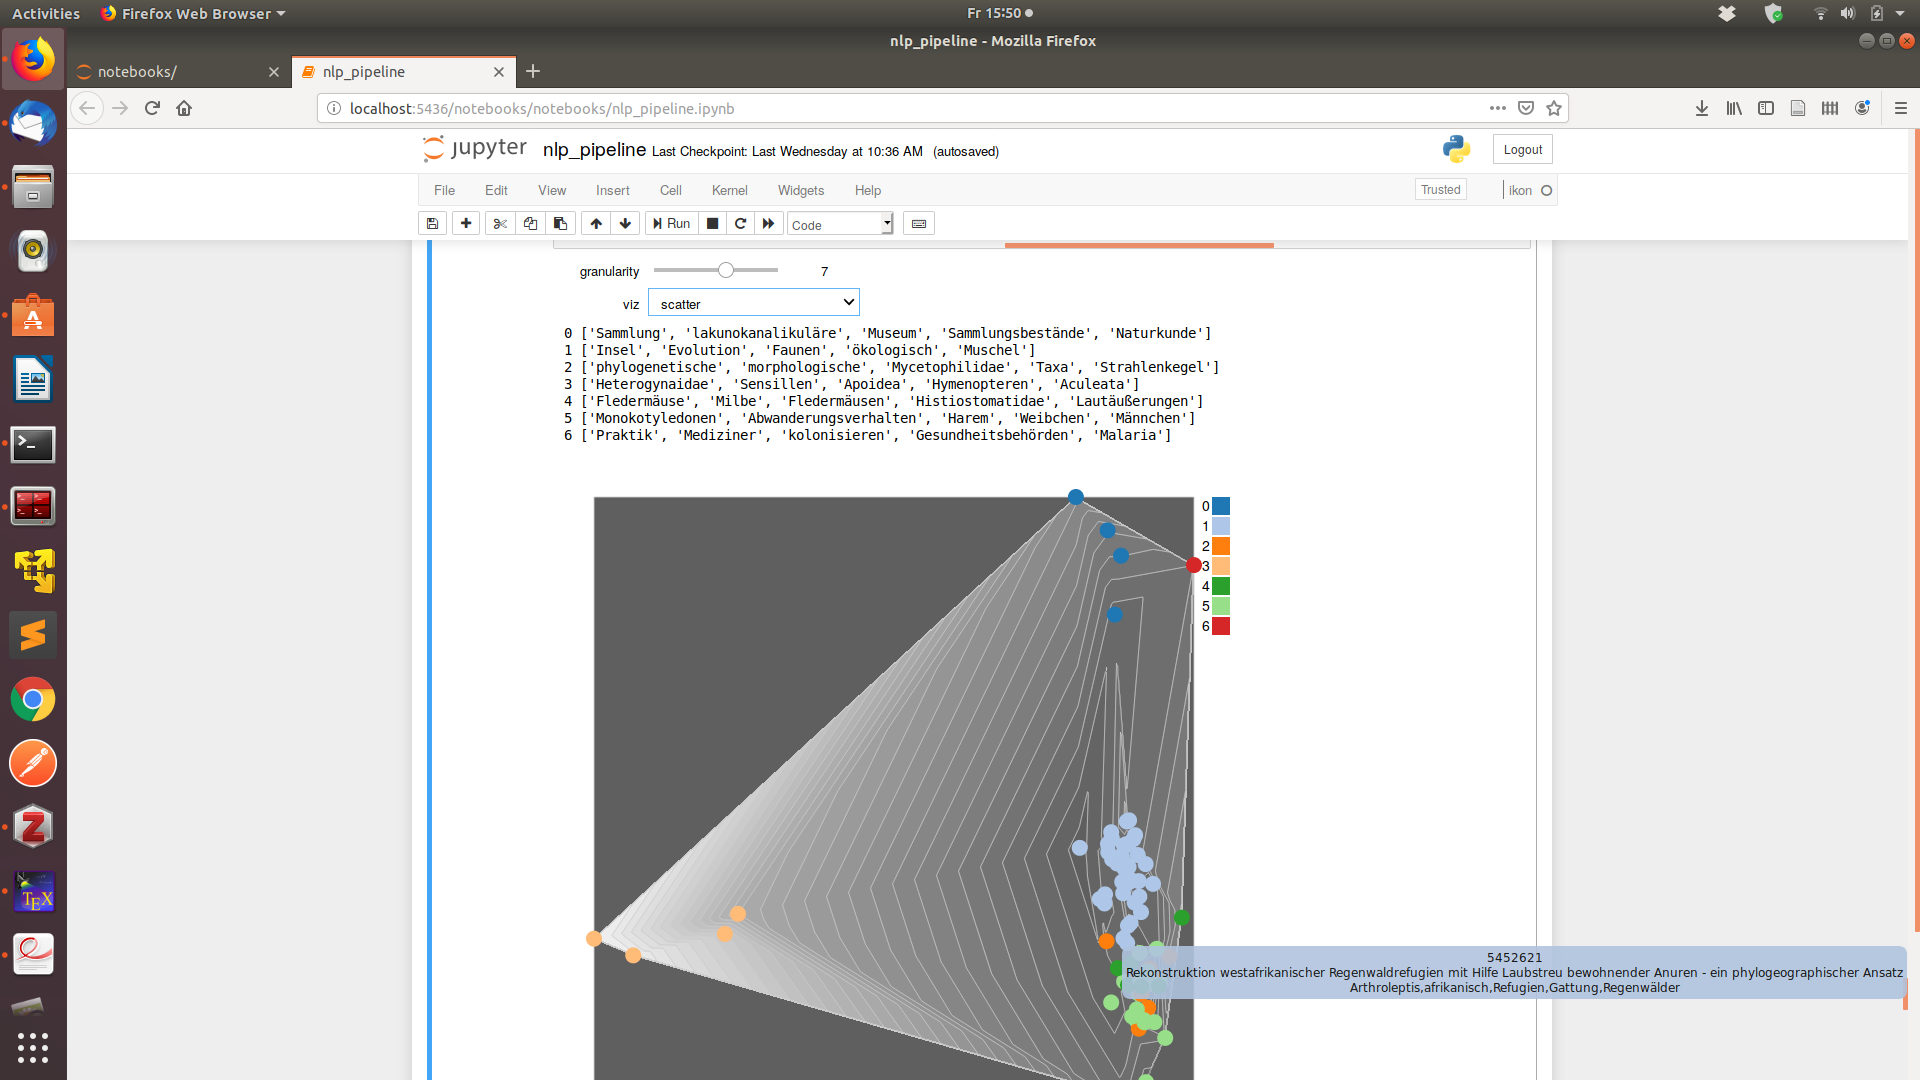
\includegraphics[width=400px]{../chapters/validation/pics/4}
	\caption{\label{pic:step4} Cognitive Walkthrough step 4}
\end{figure}

\begin{figure}[t]
	\centering
	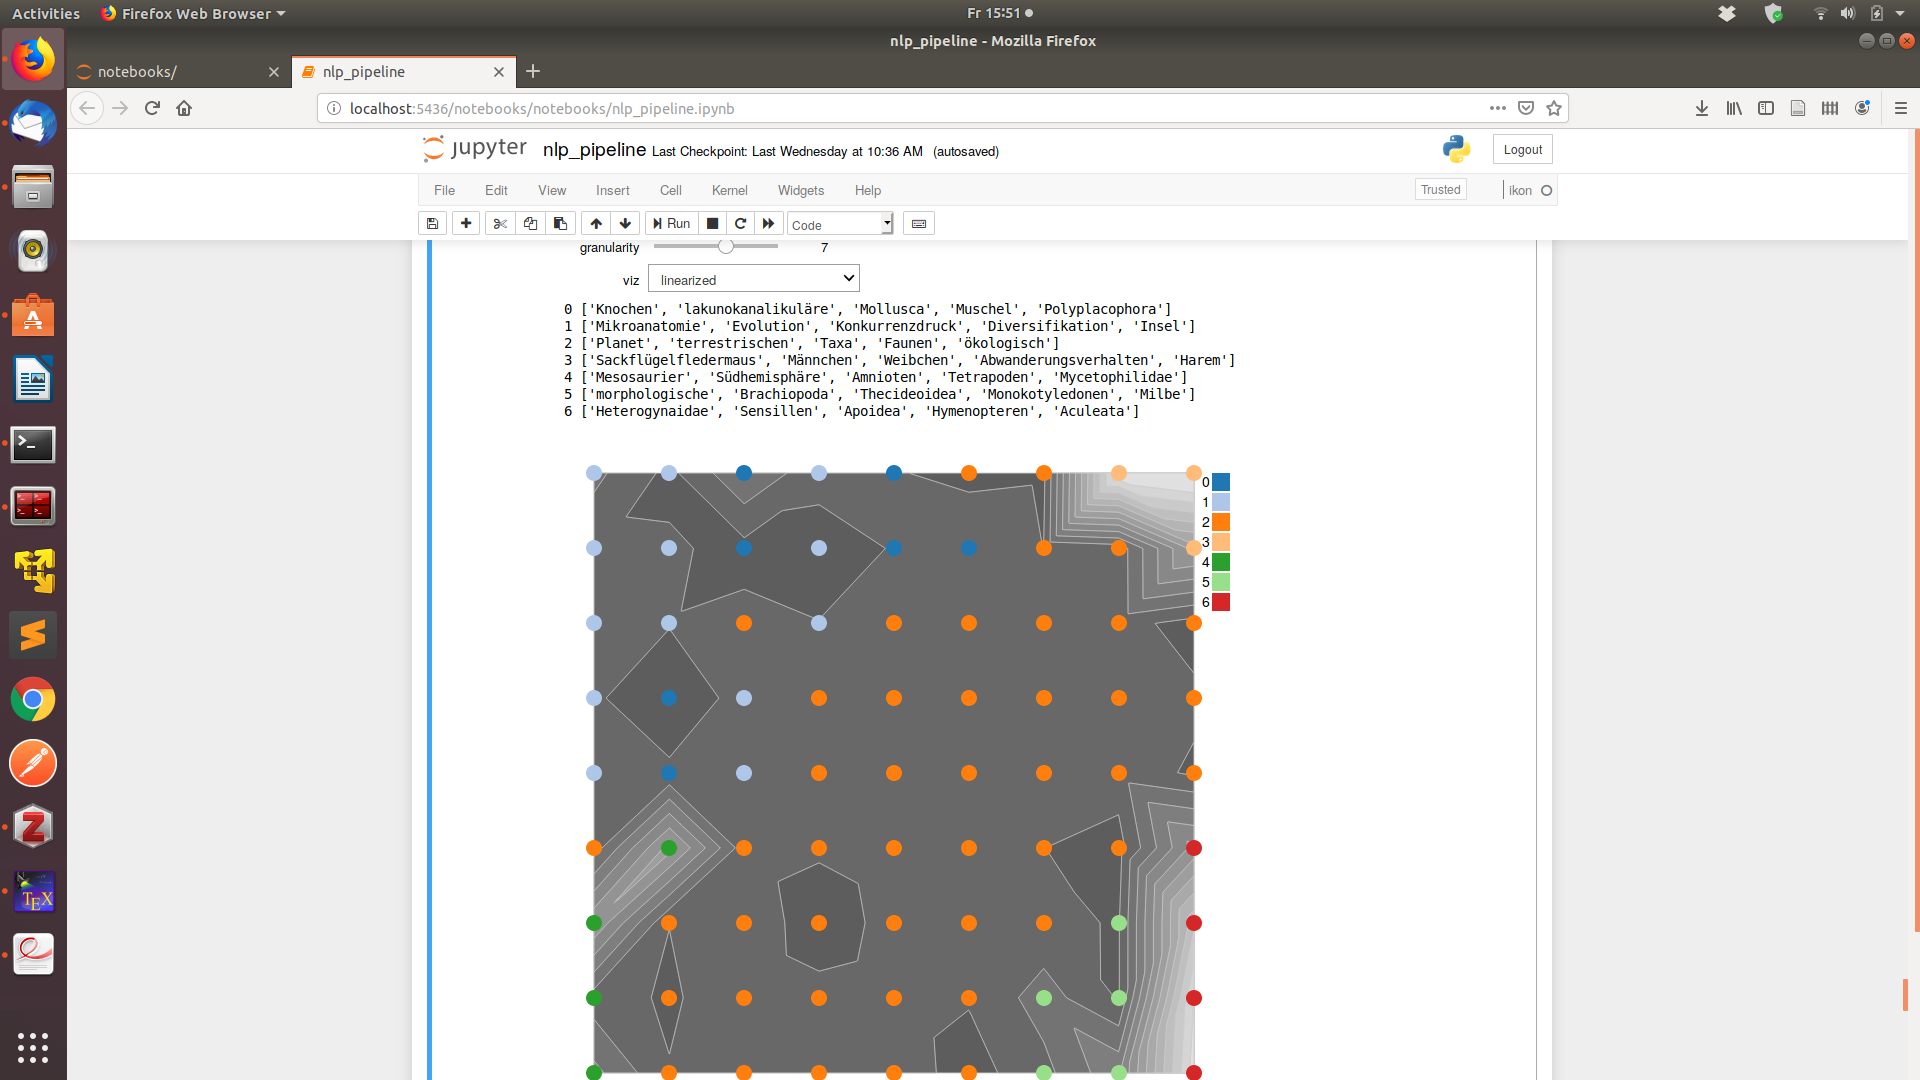
\includegraphics[width=400px]{../chapters/validation/pics/5}
	\caption{\label{pic:step5} Cognitive Walkthrough step 5}
\end{figure}

\begin{figure}[t]
	\centering
	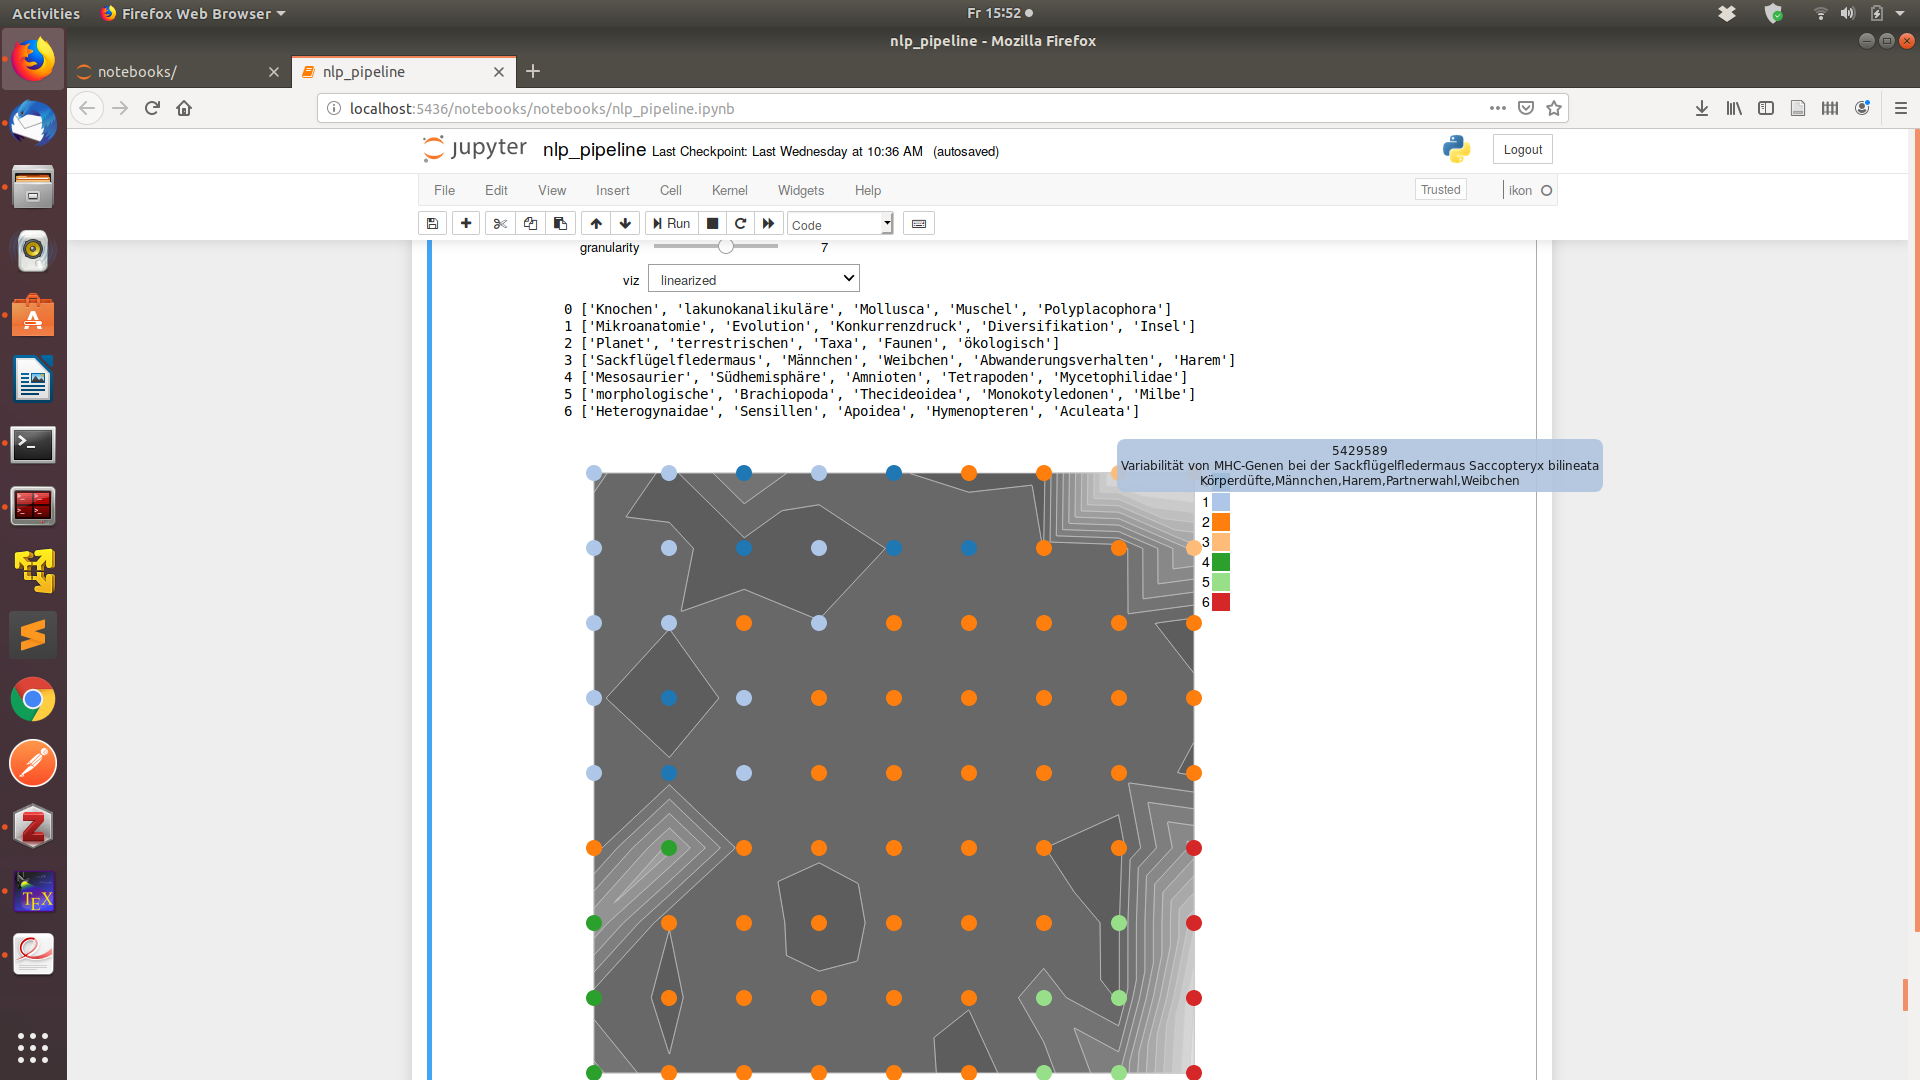
\includegraphics[width=400px]{../chapters/validation/pics/6}
	\caption{\label{pic:step6} Cognitive Walkthrough step 6}
\end{figure}

\begin{figure}[t]
	\centering
	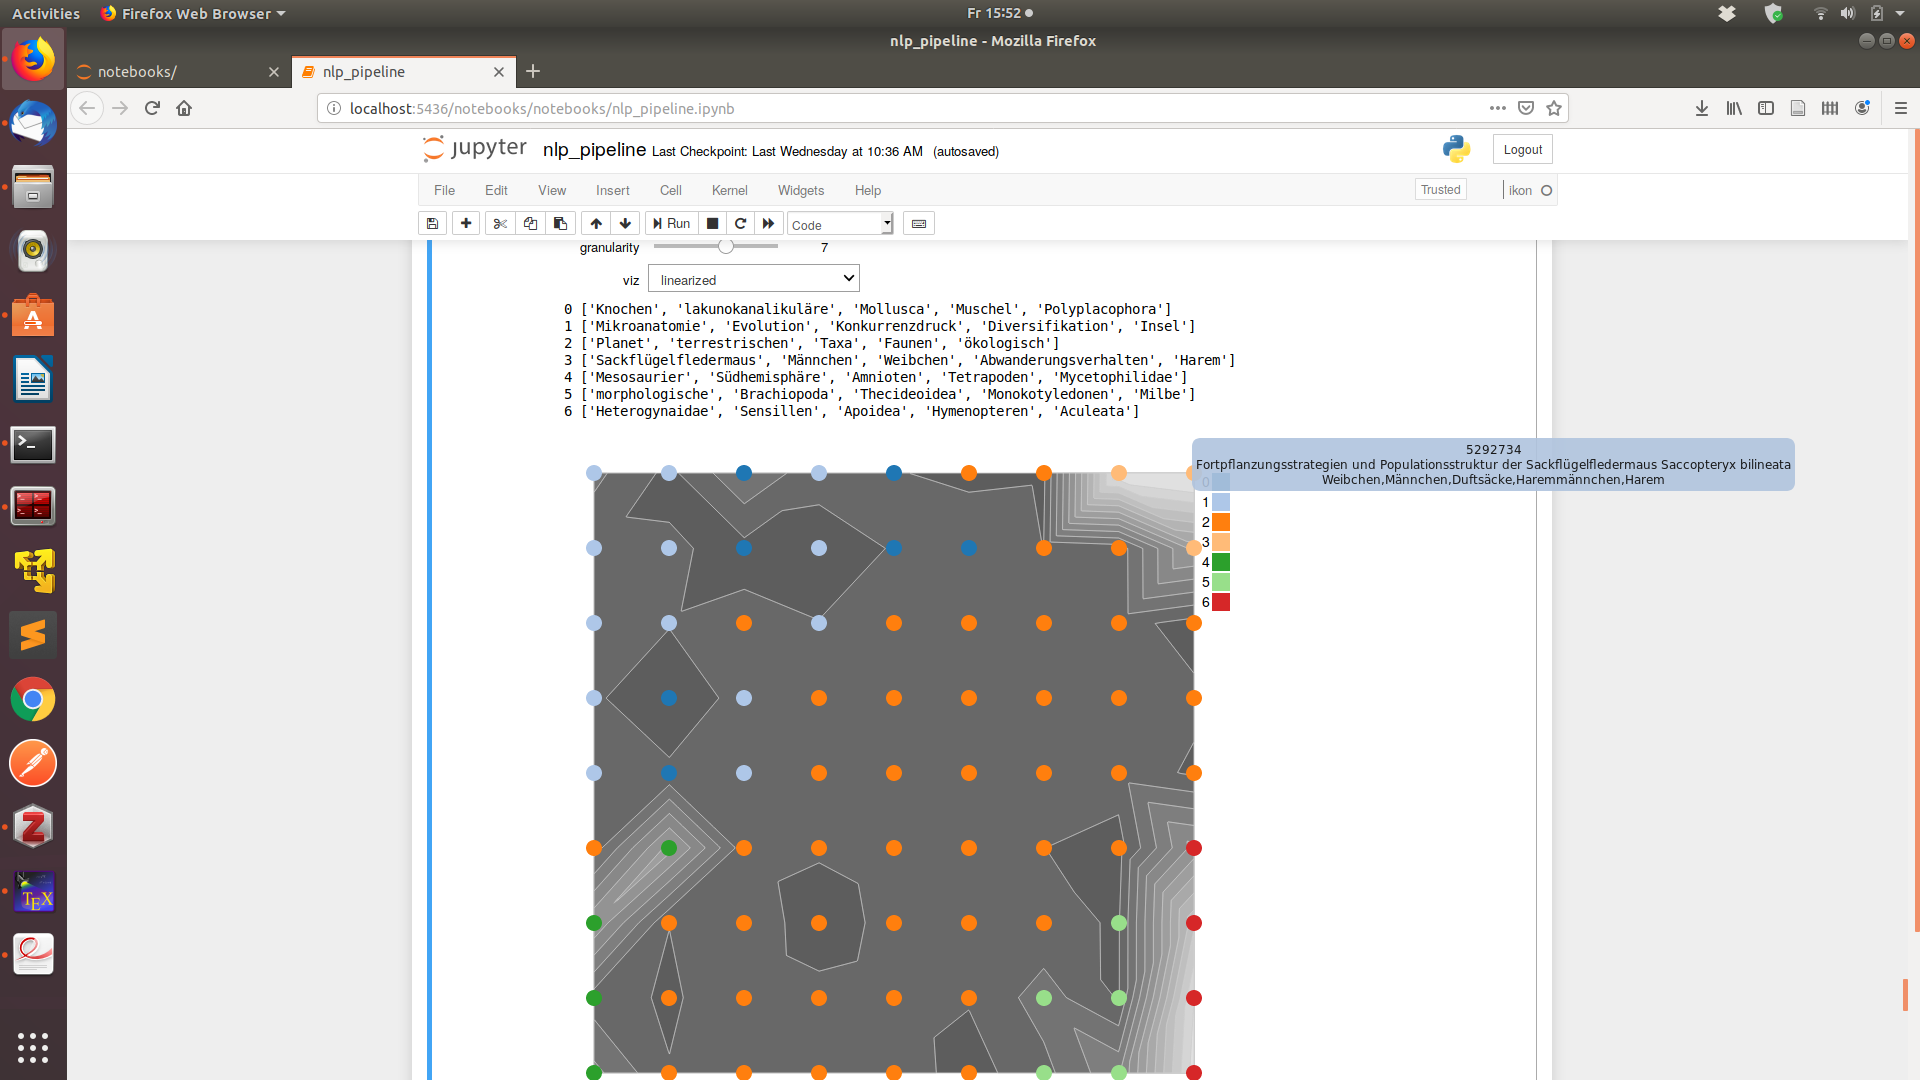
\includegraphics[width=400px]{../chapters/validation/pics/7}
	\caption{\label{pic:step7} Cognitive Walkthrough step 7}
\end{figure}

\begin{figure}[t]
	\centering
	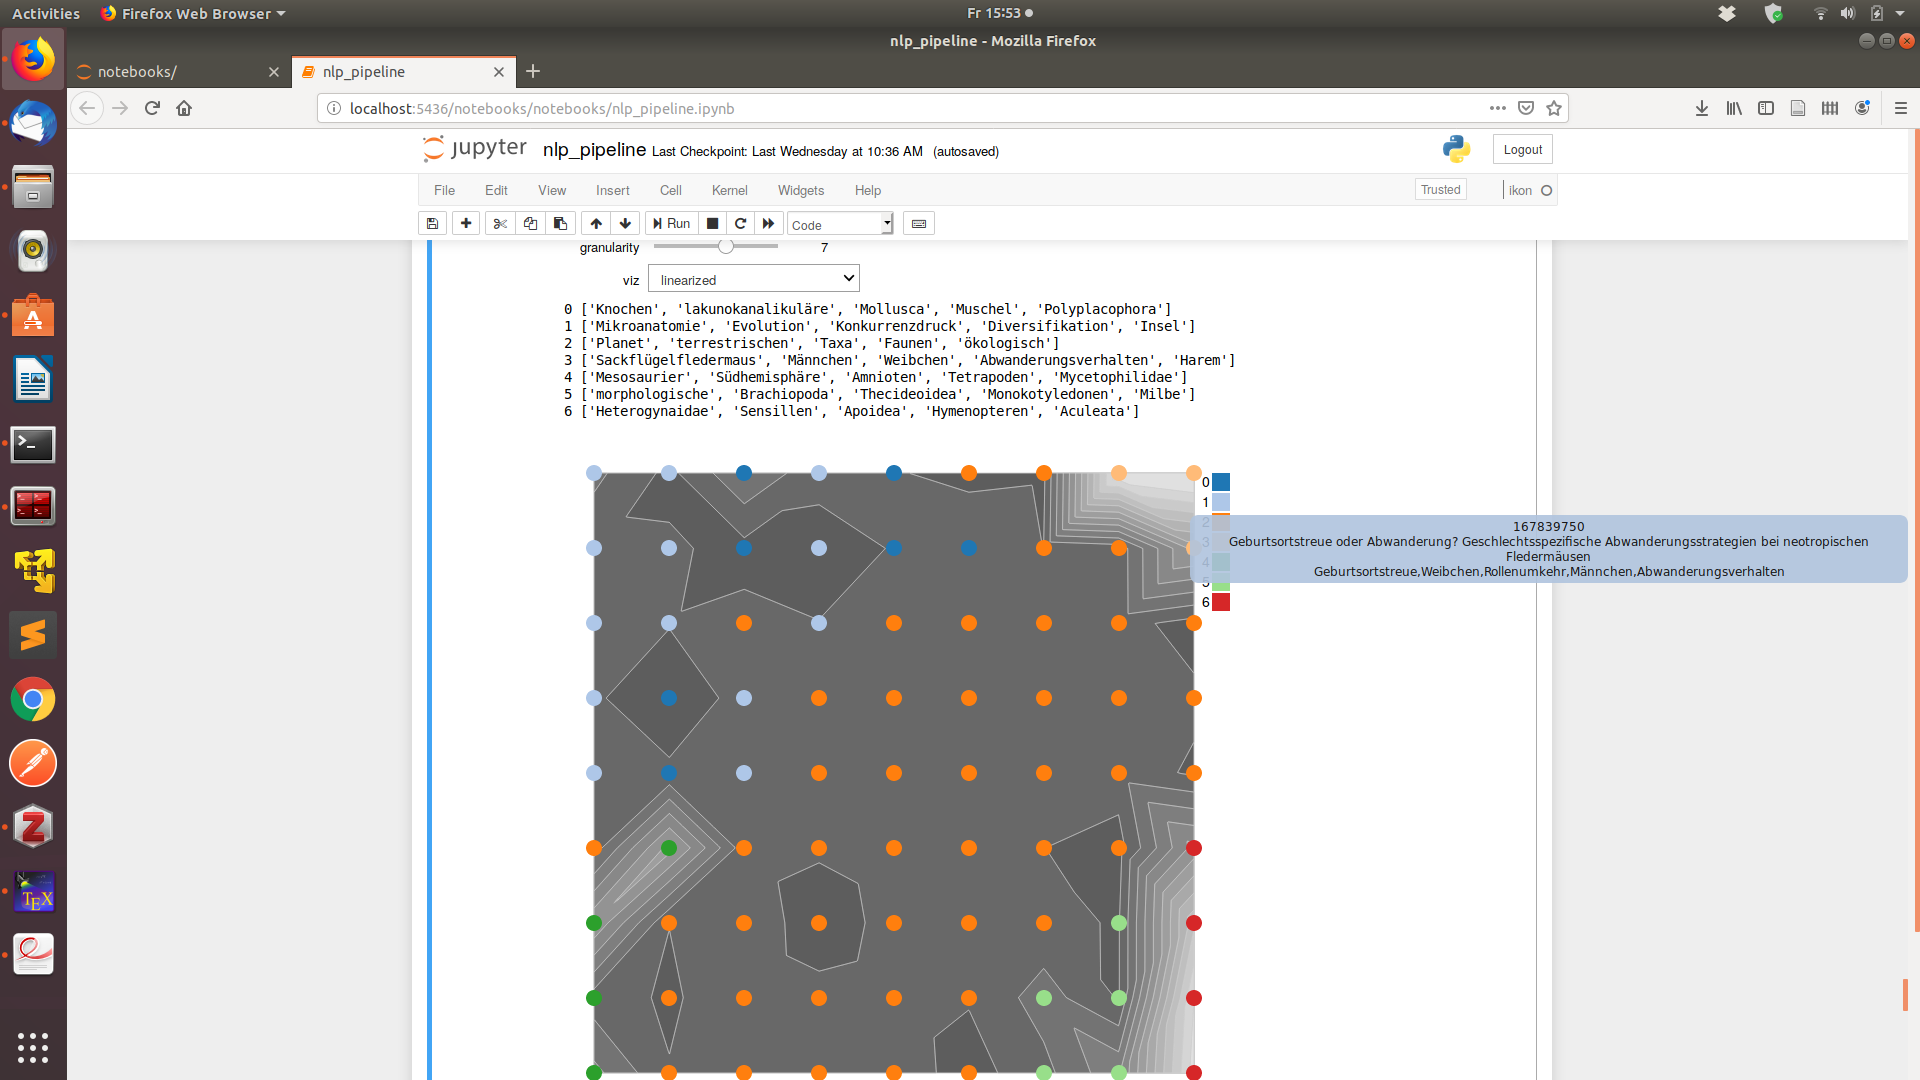
\includegraphics[width=400px]{../chapters/validation/pics/8}
	\caption{\label{pic:step8} Cognitive Walkthrough step 8}
\end{figure}

\begin{figure}[t]
	\centering
	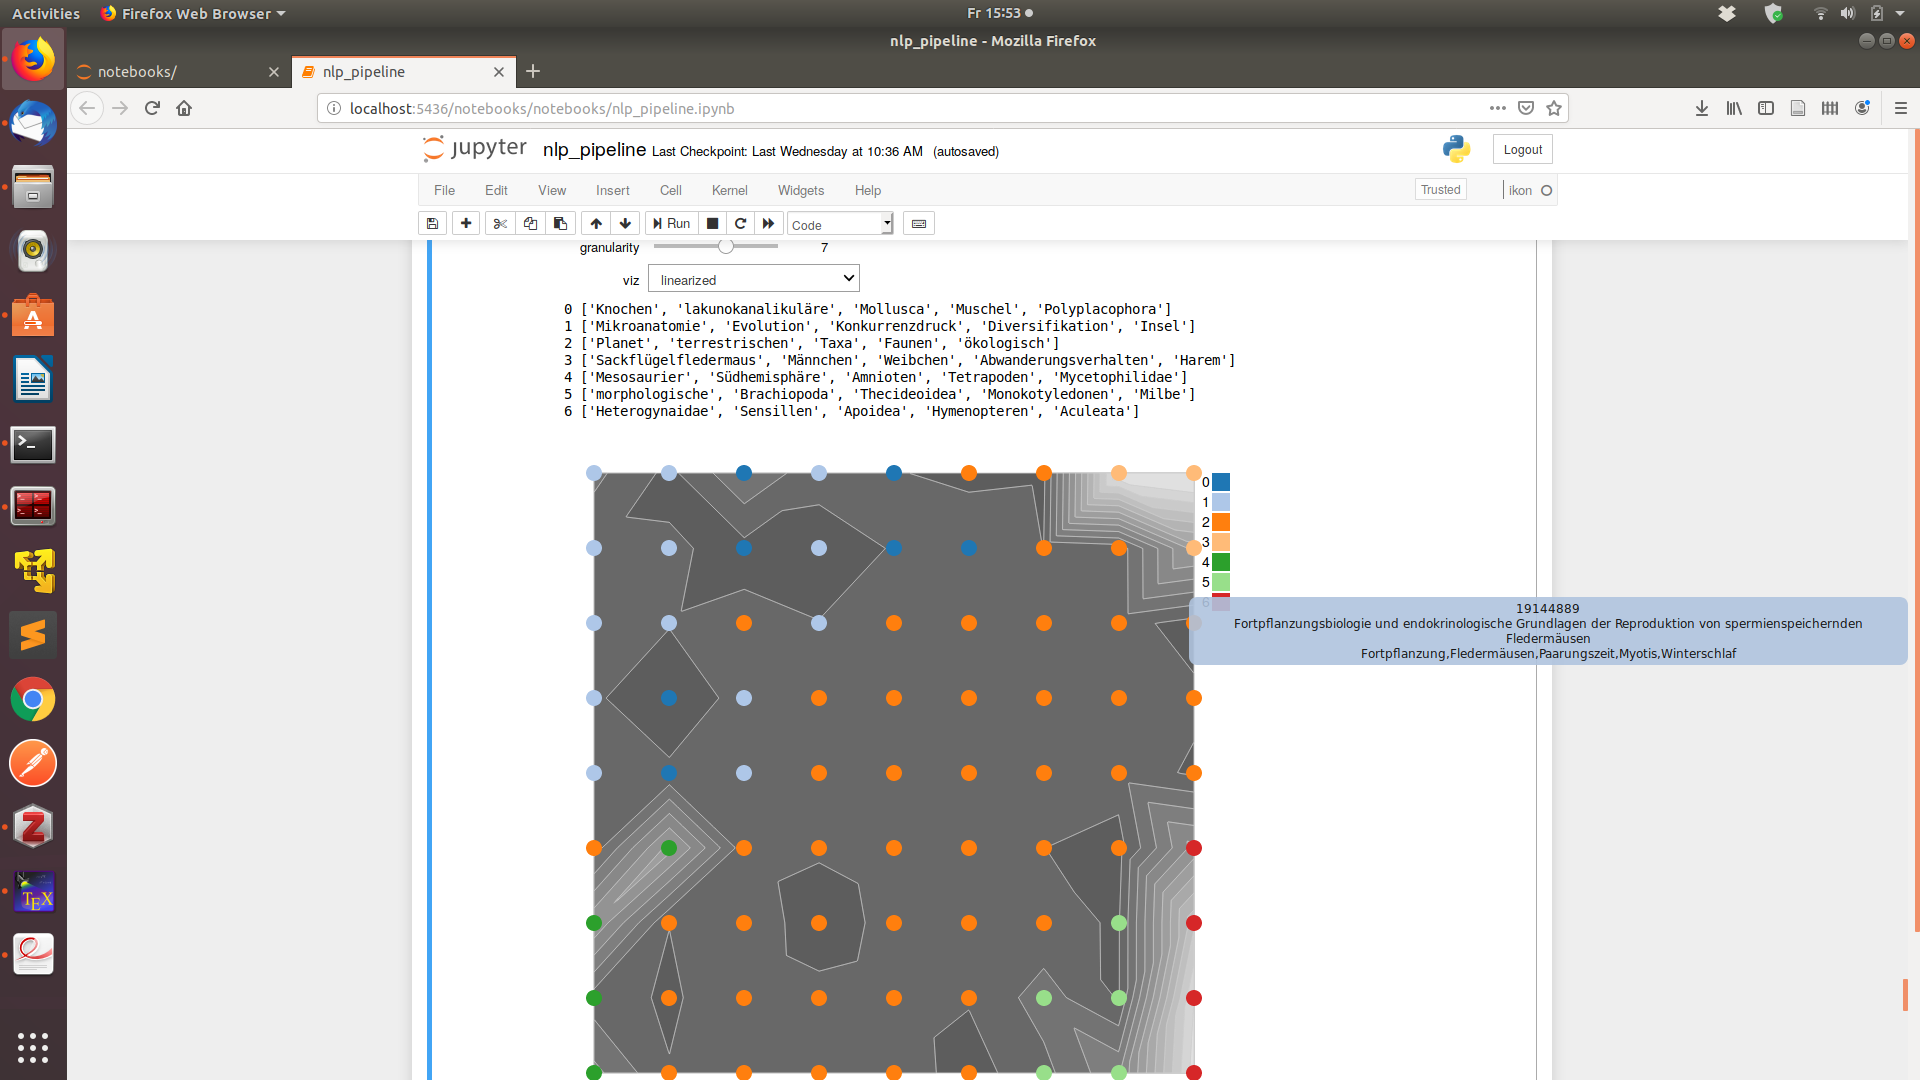
\includegraphics[width=400px]{../chapters/validation/pics/9}
	\caption{\label{pic:step9} Cognitive Walkthrough step 9}
\end{figure}

\begin{figure}[t]
	\centering
	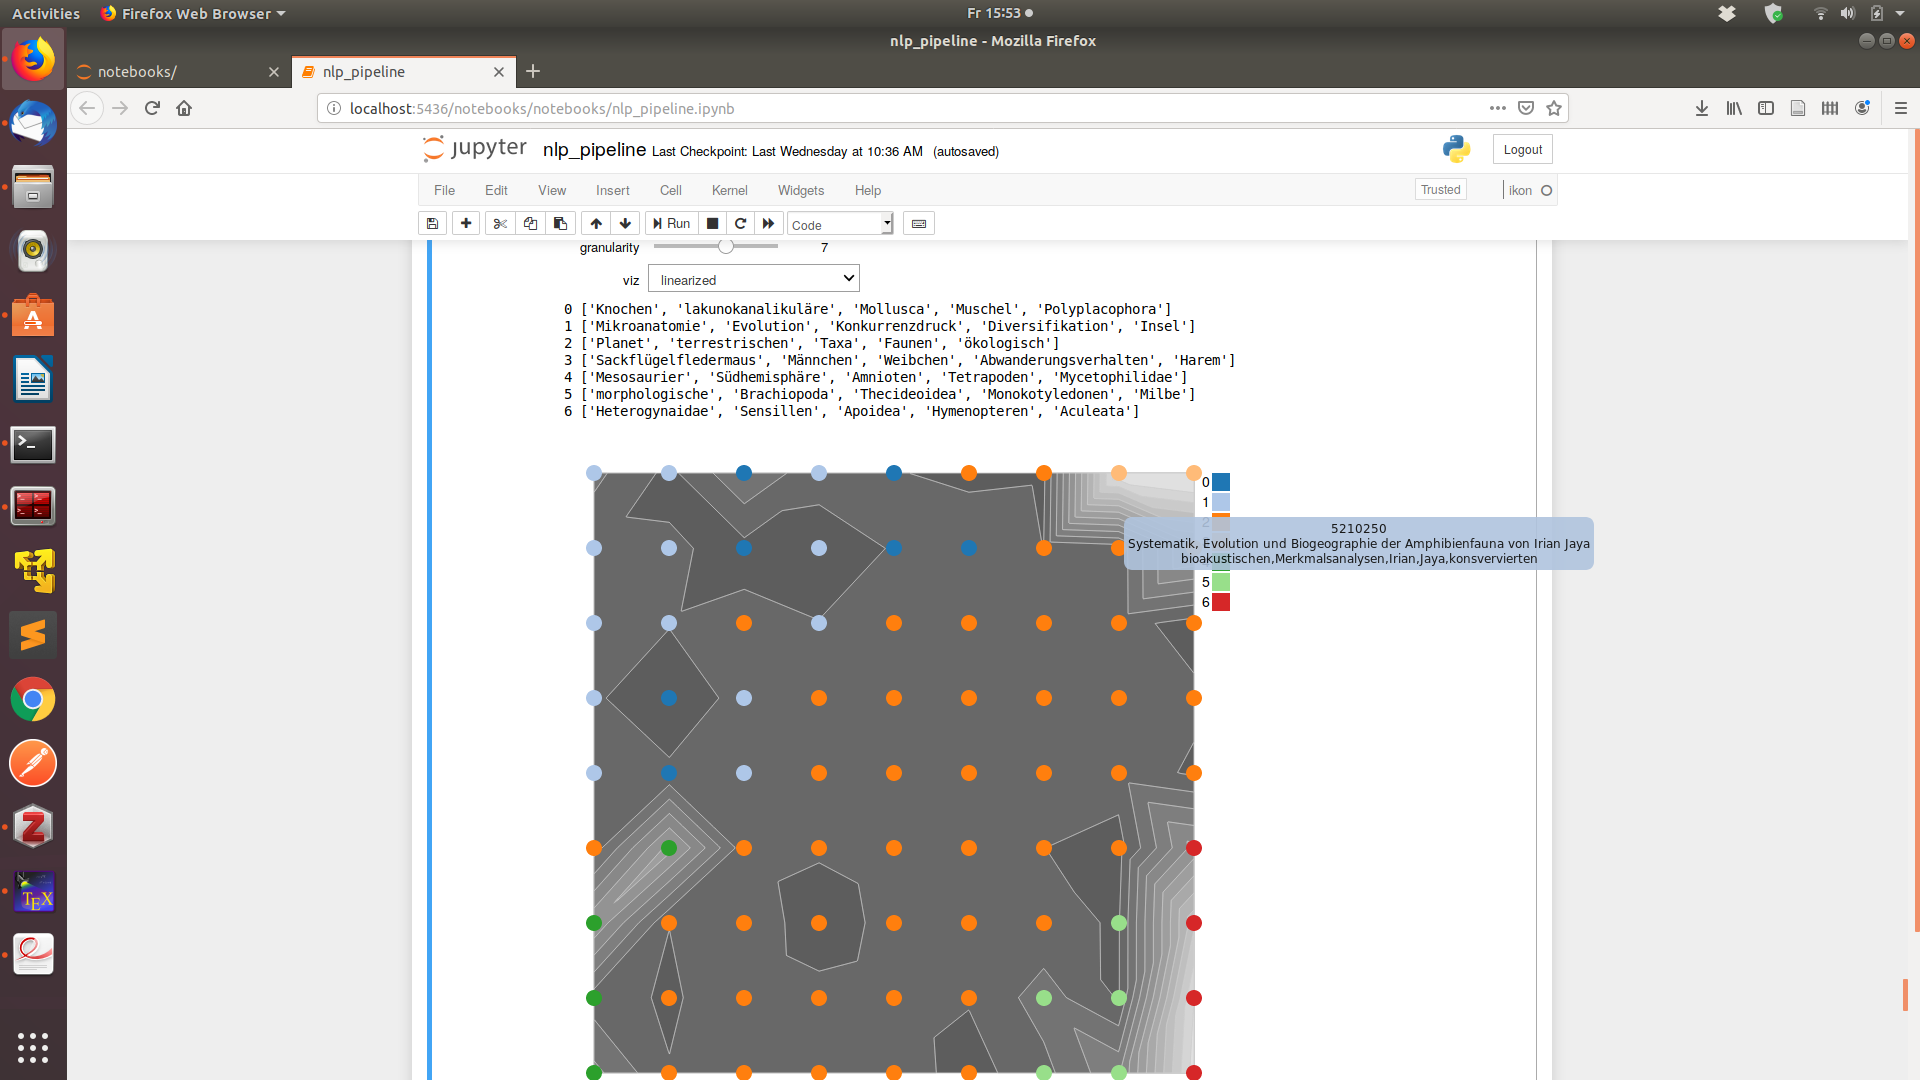
\includegraphics[width=400px]{../chapters/validation/pics/10}
	\caption{\label{pic:step10} Cognitive Walkthrough step 10}
\end{figure} 



\end{document}